% !TEX root = ../main.tex

%----------------------------------------------------------------------------------------
% APPENDIX A
%----------------------------------------------------------------------------------------

\chapter{Extra Notes on Deep Learning and materials} % Main appendix title

\label{AppendixA} % For referencing this appendix elsewhere, use \ref{AppendixA}

\section{Simple multilayer perceptron}

\begin{figure}[h]
	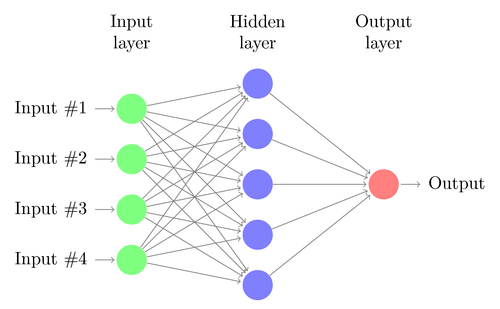
\includegraphics[width=0.75\textwidth]{../Figures/neural-network.png}
%	\centering
	\caption[An ANN]{A simple depiction of an artificial neural network} \url{https://texample.net/tikz/examples/neural-network/}
\label{fig:appendix-mlp}
\end{figure}

\begin{equation*}
	y =  \sigma\left(\sum WX + B\right)
\end{equation*}
Where
\begin{align*}
	y &  \text{ is the output or hidden layer} \\
	\sigma &  \text{is the activation function} \\
	X &  \text{ is the input vector} \\
	W &  \text{ is the weight vector} \\
	B &  \text{ Bias}
\end{align*}
Where Edges are weights and nodes are the sum of the weights *inputs + bias. An activation function like sigmoid or ReLu (which performs a kind of smooth mapping) is applied to this sum.

%\section{How can I add a Figure in the Appendix?}
%
%You can refer to a figure in the Appendix (like \ref{fig:appendix-figure}) and it will show up as expected.
%
%\begin{figure}
%\includegraphics[width=0.25\textwidth]{../Figures/Bart_Simpson.png}
%\centering
%\caption[A random appendix figure]{Bart Simpson. (2023, May 17). In Wikipedia. \url{https://en.wikipedia.org/wiki/Bart_Simpson}}
%\label{fig:appendix-figure}
%\end{figure}
